\documentclass[11pt]{article}

\usepackage[a4paper,margin=1in]{geometry}
\usepackage[T1]{fontenc}
\usepackage{lmodern}
\usepackage{booktabs}
\usepackage{longtable}
\usepackage{array}
\usepackage{enumitem}
\usepackage{float}
\usepackage{graphicx}
\usepackage[hidelinks]{hyperref}
\usepackage{xcolor}
\usepackage{listings}
\setlength{\emergencystretch}{3em}
\graphicspath{{evidence-screenshots/}}

\lstdefinestyle{sentinel}{
  basicstyle=\ttfamily\small,
  breaklines=true,
  frame=single,
  columns=fullflexible,
  keepspaces=true
}

\title{Sentinel: A Functional Signature-Based Virus Scanner}
\author{513559004 Jsaon Chia-Sheng Lin; 313264012 Ching-Chung Chen}
\date{2026-04-22}

\begin{document}
\maketitle

\section*{Abstract}

Sentinel is a safe, read-only, signature-based virus scanner for the Network
Security Practice final project. It scans an explicit target directory, loads a
structured malware-signature database, combines Bloom-filter hash pre-checks
with exact hash-map verification, performs Aho-Corasick byte-pattern matching,
skips symbolic links by default, separates heuristic warnings from confirmed
signature matches, and generates JSON and Markdown evidence reports. The demo
uses only local safe fixtures, not live malware.

\section{Team And Submission Decisions}

This report covers Project I - Virus Scanner. The recorded team members are
513559004 Jsaon Chia-Sheng Lin and 313264012 Ching-Chung Chen.

The implementation is not moved into a private GitHub or GitLab repository in
this pass, by instruction. The private repository URL is therefore recorded as
not created or moved. The local demo commit hash for the current package is
\texttt{2be51a0f003834e58795efcdd4b9224a730b90e7}. The current final demo does
not require the literal EICAR test file; it uses a safe mock fixture plus EICAR
reference hashes unless the instructor explicitly requires literal EICAR later.

\section{Introduction}

The project goal is to identify a known mock threat hidden inside a directory
tree and produce a clear security report. Sentinel is intentionally educational:
it does not execute scanned files, delete files, quarantine files, upload files,
or scan the whole machine by default. The current demo uses a local safe
mock-virus marker rather than live malware or the literal EICAR string. If the
instructor requires the exact EICAR test file, it should be created only in the
controlled final demo environment and recorded in the final evidence manifest.

\section{Requirement Mapping}

\begin{longtable}{p{0.33\linewidth}p{0.57\linewidth}}
\toprule
\textbf{Official requirement} & \textbf{Sentinel implementation} \\
\midrule
Structured malware-signature repository &
\texttt{signatures/malware-signatures.json} stores MD5, SHA-256, and
hex-pattern matchers. \\
File traversal and comparison &
\texttt{sentinel.scanner} walks the explicit target directory in sorted order
and scans regular files. \\
Bitwise or pattern comparison &
\texttt{hex\_pattern} signatures are converted to bytes and searched during
chunked file scans using an Aho-Corasick byte-pattern automaton. \\
Heuristic analysis &
\texttt{sentinel.heuristics} flags low-confidence suspicious indicators without
claiming confirmed infection. \\
Security report &
\texttt{sentinel.reporting} writes timestamped JSON and Markdown reports with
paths, statuses, severities, hashes, and evidence. \\
Demonstration &
\texttt{demo/demo-tree/} contains clean files, one safe mock-virus fixture, and
one heuristic-only suspicious fixture. \\
\bottomrule
\end{longtable}

\section{Signature Database Design}

The signature database uses JSON because it is easy to inspect, easy to validate
with the Python standard library, and flexible enough to support multiple
matcher types per signature. Each signature has a stable identifier, name,
category, severity, matchers, and optional notes.

The current safe mock-virus signature uses three matchers:

\begin{center}
\begin{tabular}{ll}
\toprule
\textbf{Matcher} & \textbf{Purpose} \\
\midrule
\texttt{md5} & Fast exact-file detection for the known demo fixture. \\
\texttt{sha256} & Stronger exact-file detection for the known demo fixture. \\
\texttt{hex\_pattern} & Byte-pattern matching for the bitwise comparison requirement. \\
\bottomrule
\end{tabular}
\end{center}

\subsection{Data Structures}

\begin{longtable}{p{0.34\linewidth}p{0.24\linewidth}p{0.32\linewidth}}
\toprule
\textbf{Structure} & \textbf{Purpose} & \textbf{Reason} \\
\midrule
\texttt{tuple[Signature, ...]} & Validated signature records &
Keeps the loaded database stable during a scan. \\
\texttt{dict[str, dict[str, tuple[HashMatcher, ...]]]} & Hash lookup by
algorithm and digest & Exact hash detection becomes a constant-time dictionary
lookup. \\
\texttt{HashBloomFilter} & Hash membership pre-check & Avoids unnecessary exact
hash-map checks while preserving exact verification for possible hits. \\
\texttt{PatternScanEngine} & Aho-Corasick byte-pattern automaton & Reused across
files during a scan run. \\
\texttt{PatternStreamScanner} & Per-file automaton state & Preserves pattern
state across streamed chunks. \\
\texttt{list[HeuristicFinding]} & Suspicious-rule output & Keeps heuristic
signals separate from confirmed signature matches. \\
\bottomrule
\end{longtable}

The Bloom filter stores normalized \texttt{algorithm:digest} keys for configured
hash signatures. It answers only ``might contain.'' Sentinel then confirms every
possible hit against the exact hash map, so Bloom-filter false positives cannot
create infected results.

\section{Scanning Engine}

The scanner workflow is:

\begin{enumerate}[leftmargin=*]
  \item Parse CLI arguments.
  \item Load and validate the signature database.
  \item Walk the explicit target directory in sorted order.
  \item Report symbolic links as \texttt{skipped} rather than following them.
  \item Read each file in chunks.
  \item Compute MD5 and SHA-256 incrementally.
  \item Pre-check hash signatures through the Bloom filter.
  \item Confirm possible hash hits through exact lookup maps.
  \item Search configured byte patterns with an Aho-Corasick automaton.
  \item Run heuristic rules against a bounded sample.
  \item Assign status: \texttt{infected}, \texttt{suspicious}, \texttt{clean},
        \texttt{skipped}, or \texttt{error}.
  \item Write JSON or Markdown report output.
\end{enumerate}

Chunked scanning avoids loading full files into memory for hash and pattern
matching. For byte-pattern matching, Sentinel builds a trie with failure links
from all configured patterns, then feeds file chunks through one automaton state
machine. This means a signature split across two chunks is still detectable
without manually searching each pattern against each chunk. The overlapping,
stream-boundary, and chunk-boundary pattern tests verify this behavior.

\subsection{Algorithmic Hardening}

The pattern engine uses the Aho-Corasick idea: multiple patterns are compiled
into one automaton, and each input byte advances one shared state machine. The
JSON report records \texttt{hash\_filter}, \texttt{hash\_filter\_policy},
\texttt{pattern\_engine}, \texttt{pattern\_count}, \texttt{automaton\_states},
chunk-size metadata, and \texttt{symlink\_policy} so the demo evidence shows
which matching and traversal paths were used.

The benchmark in \texttt{reports/pattern-benchmark.json} is safe and synthetic.
It compares the automaton with a naive per-pattern \texttt{bytes} search. The
current benchmark shows equal match sets. It does not claim production antivirus
performance; in small Python-only demos, CPython's C-backed byte search can be
faster than a pure-Python automaton. The professional value here is explainable
multi-pattern behavior and scaling structure.

The scanner returns exit code \texttt{1} when an infected file is found. In the
demo this is expected because the safe mock-virus fixture is intentionally
detected.

\section{Heuristic Analysis}

Heuristics are deliberately separated from signatures. A heuristic-only hit is
reported as \texttt{suspicious}, not \texttt{infected}. This avoids overstating
weak evidence.

\begin{longtable}{p{0.28\linewidth}p{0.36\linewidth}p{0.26\linewidth}}
\toprule
\textbf{Rule} & \textbf{Signal} & \textbf{Limitation} \\
\midrule
\texttt{api-name} & Safe fixture mentions API names such as
\texttt{CreateRemoteThread}, \texttt{VirtualAllocEx}, and
\texttt{WriteProcessMemory}. & String presence alone does not prove malware. \\
\texttt{magic-mismatch} & A \texttt{.txt} file begins with
executable-like \texttt{MZ} bytes. & Benign mislabeled files can exist. \\
\texttt{high-entropy} & A small binary-like file has high byte
entropy. & Compressed benign files may also trigger. \\
\bottomrule
\end{longtable}

\section{Report And Evidence Artifacts}

Sentinel currently generates:

\begin{itemize}[leftmargin=*]
  \item \texttt{reports/demo-report.json}: machine-readable scan report.
  \item \texttt{reports/demo-report.md}: instructor-friendly Markdown report.
  \item \texttt{reports/pattern-benchmark.json}: safe synthetic benchmark data.
  \item \texttt{reports/pattern-benchmark.md}: benchmark summary.
  \item \texttt{reports/demo-evidence-manifest.json}: reproducibility manifest.
\end{itemize}

The evidence manifest records SHA-256 hashes and sizes for every demo-tree file,
the signature database, generated reports, and benchmark artifacts. It also
records the safety flags and exact commands used to reproduce the evidence.

\section{External Standards Alignment}

The project was calibrated against a small set of recognized references:
EICAR/CARO for safe anti-malware testing, NIST SP 800-83 Rev. 1 for malware
prevention and handling, NIST Cybersecurity Framework 2.0 for risk-management
framing, OWASP File Upload guidance for defense-in-depth around untrusted files,
and MITRE ATT\&CK T1055.002 for process-injection API context. The mapping is
recorded in \texttt{docs/standards-alignment.md}.

Sentinel uses these references conservatively. The repository stores an EICAR
reference signature file containing only the reference MD5 and SHA-256 hashes. It
does not store the literal EICAR test file. The EICAR unit tests reconstruct the
reference bytes in memory to verify the standard 68-byte length and expected
hashes. MITRE API-name indicators are reported only as \texttt{suspicious}; they
are not treated as confirmed malware without an exact signature match.

\section{Release Readiness}

Sentinel includes \texttt{VERSION}, \texttt{CHANGELOG.md}, \texttt{Makefile},
and \texttt{scripts/check\_release.py}. The release check is intended to be run
before moving the package into the required private repository and again after
the move. It validates version consistency, standards alignment, EICAR reference
hashes, full demo regeneration, expected demo counts, Bloom-filter metadata,
Aho-Corasick metadata, symbolic-link policy, benchmark equivalence,
evidence-manifest safety flags, private-repository export boundaries, and
final-report PDF presence.

\begin{lstlisting}[style=sentinel]
PYTHONDONTWRITEBYTECODE=1 PYTHONPATH=src python3 scripts/check_release.py
\end{lstlisting}

\section{Current Evaluation}

\subsection{Demo Result}

\begin{center}
\begin{tabular}{lr}
\toprule
\textbf{Metric} & \textbf{Result} \\
\midrule
Files scanned & 5 \\
Infected & 1 \\
Suspicious & 1 \\
Clean & 3 \\
Errors & 0 \\
\bottomrule
\end{tabular}
\end{center}

The infected file is the nested Sentinel safe mock-virus fixture. It matches by
MD5, SHA-256, and hex-pattern evidence. The suspicious file is the API-name
fixture; it is marked suspicious because it contains API-name indicators, not
because it matches a confirmed malware signature.

The demo report records \texttt{bloom-filter} as the hash pre-check and states
that possible hits are verified by the exact hash map. It also records
\texttt{aho-corasick-byte-automaton} as the pattern engine, with one configured
pattern and 30 automaton states for the current signature database.

\subsection{Test Result}

The current standard-library test suite contains 25 tests. It covers signature
validation, Bloom-filter hash pre-checks, exact hash matching, Aho-Corasick
byte-pattern matching, overlapping pattern outputs, stream/chunk-boundary
pattern detection, scanner behavior, symbolic-link skipping, EICAR reference
hash validation, report generation, Markdown output, evidence manifest
generation, private-repo export boundaries, CLI paths, and the version flag.

\begin{lstlisting}[style=sentinel]
PYTHONDONTWRITEBYTECODE=1 PYTHONPATH=src python3 -m unittest discover -s tests -v
\end{lstlisting}

\clearpage
\section{Screenshot Evidence}

This report includes screenshot evidence for each primary project part: signature
database, scanner interface and core metadata, demo folder structure, scan
result, release gate, and final submission package.

\begin{figure}[H]
\centering
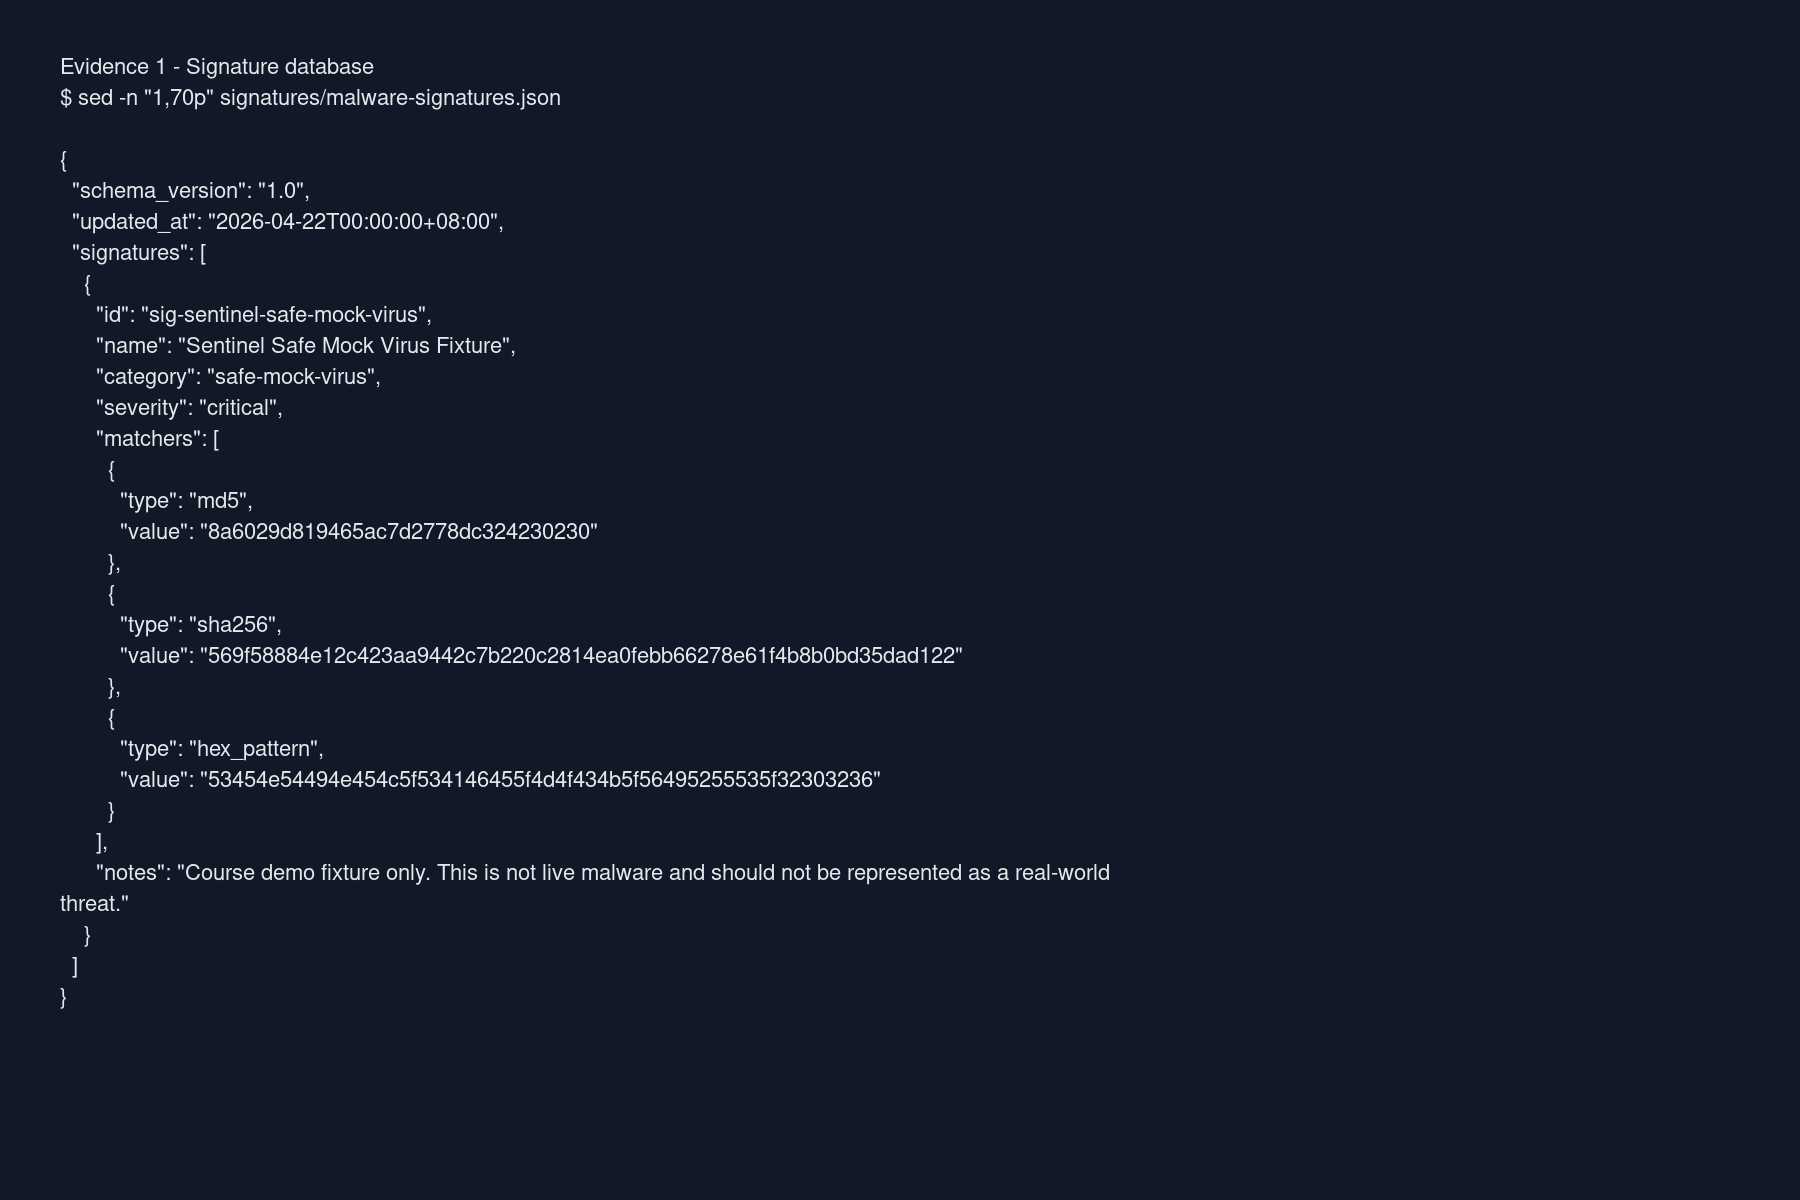
\includegraphics[width=\linewidth]{signature-database.png}
\caption{Signature database evidence showing the structured safe mock-virus signatures.}
\end{figure}
\clearpage

\begin{figure}[H]
\centering
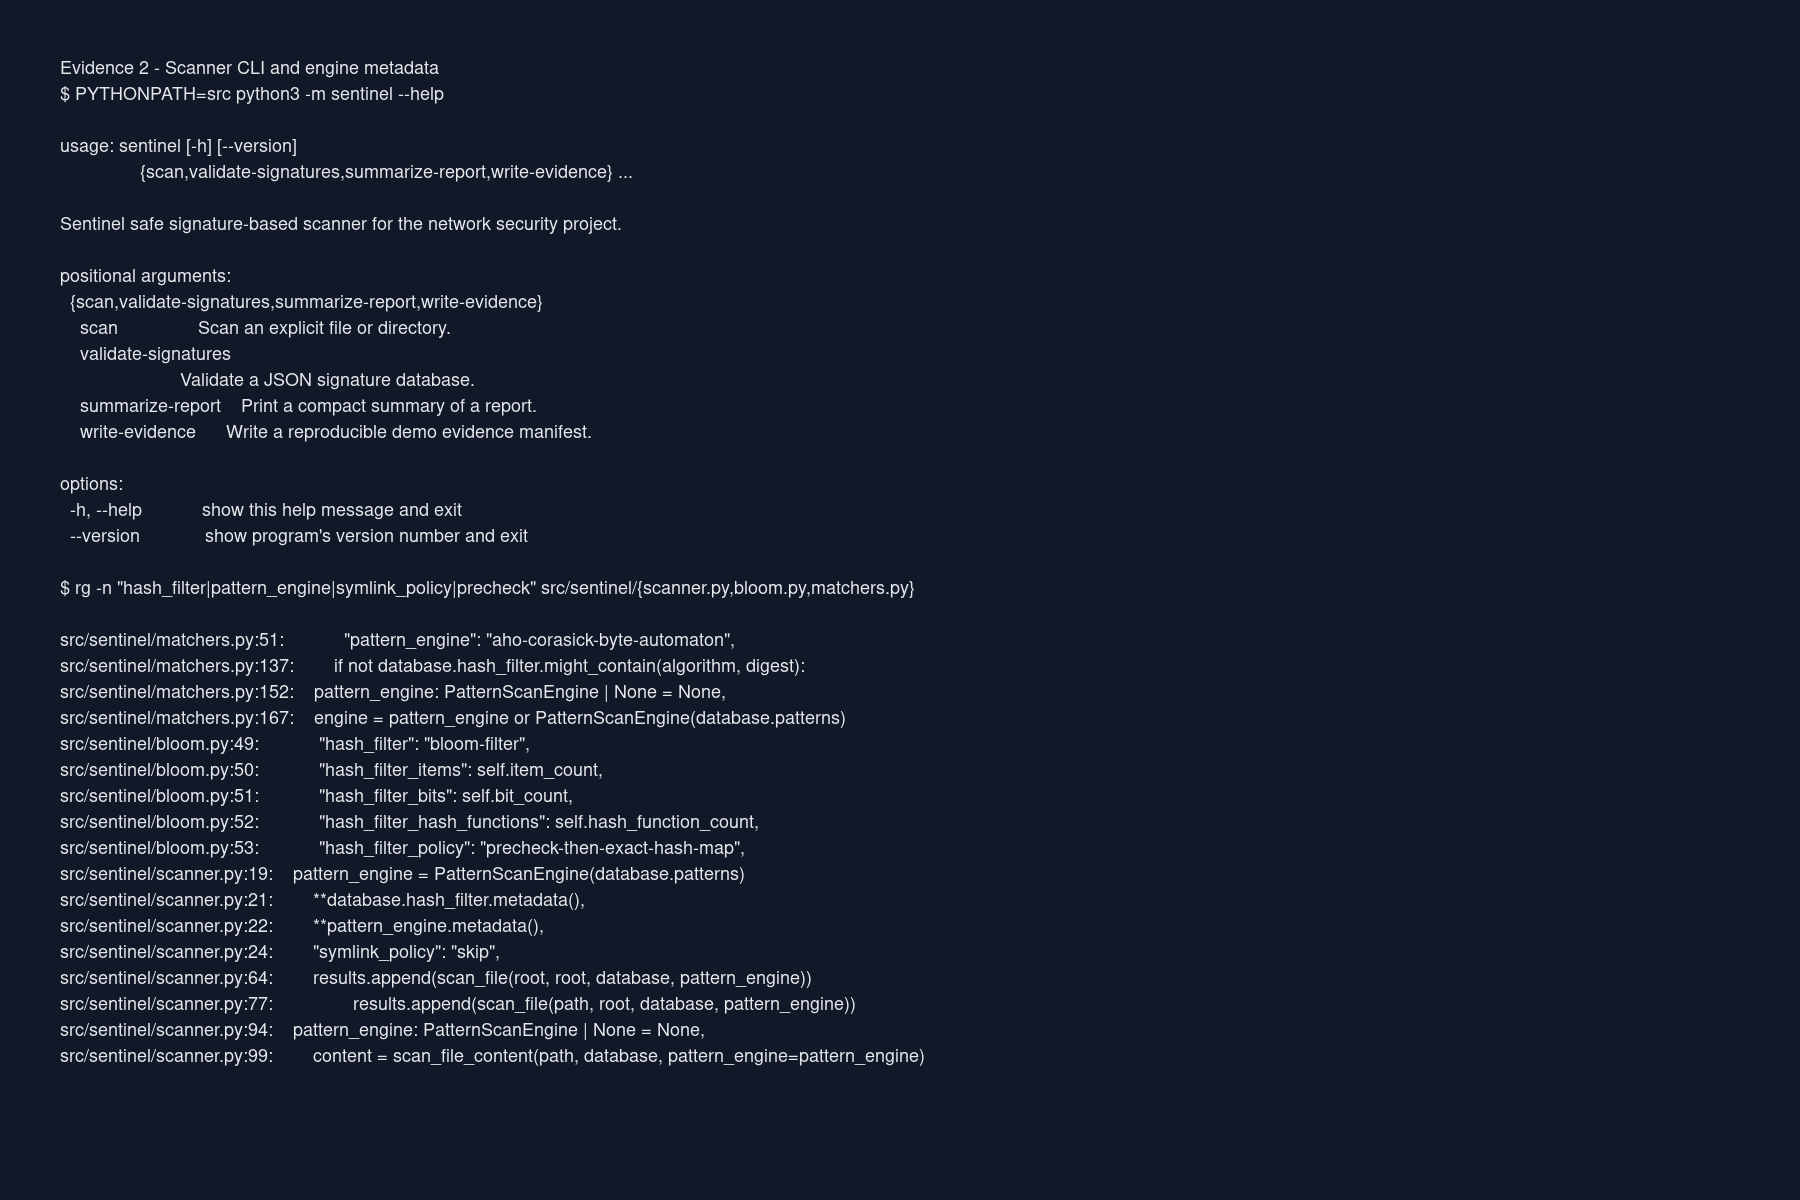
\includegraphics[width=\linewidth]{scanner-cli.png}
\caption{Scanner interface and engine metadata evidence showing the CLI and implemented hash/pattern policies.}
\end{figure}
\clearpage

\begin{figure}[H]
\centering
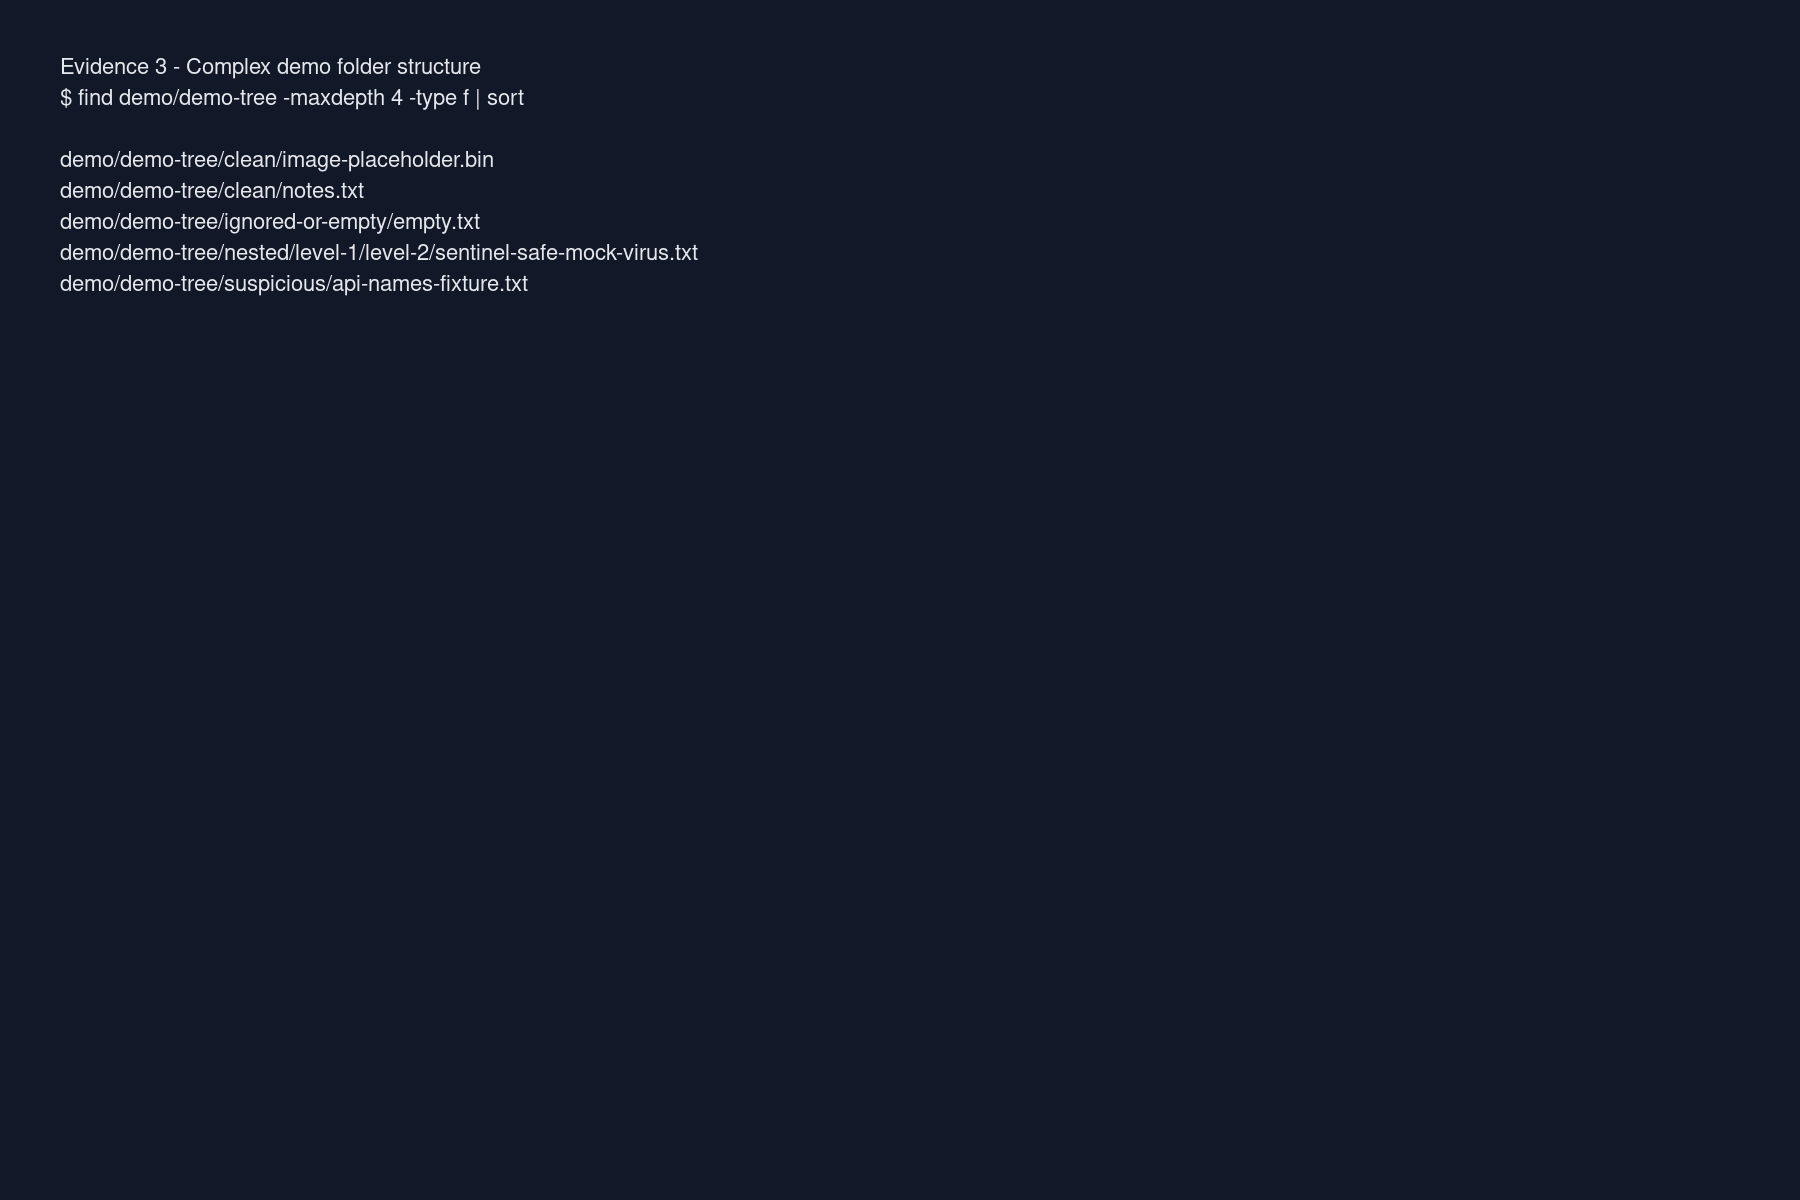
\includegraphics[width=\linewidth]{demo-tree.png}
\caption{Demo folder evidence showing clean files, nested safe mock-virus fixture, and suspicious fixture.}
\end{figure}
\clearpage

\begin{figure}[H]
\centering
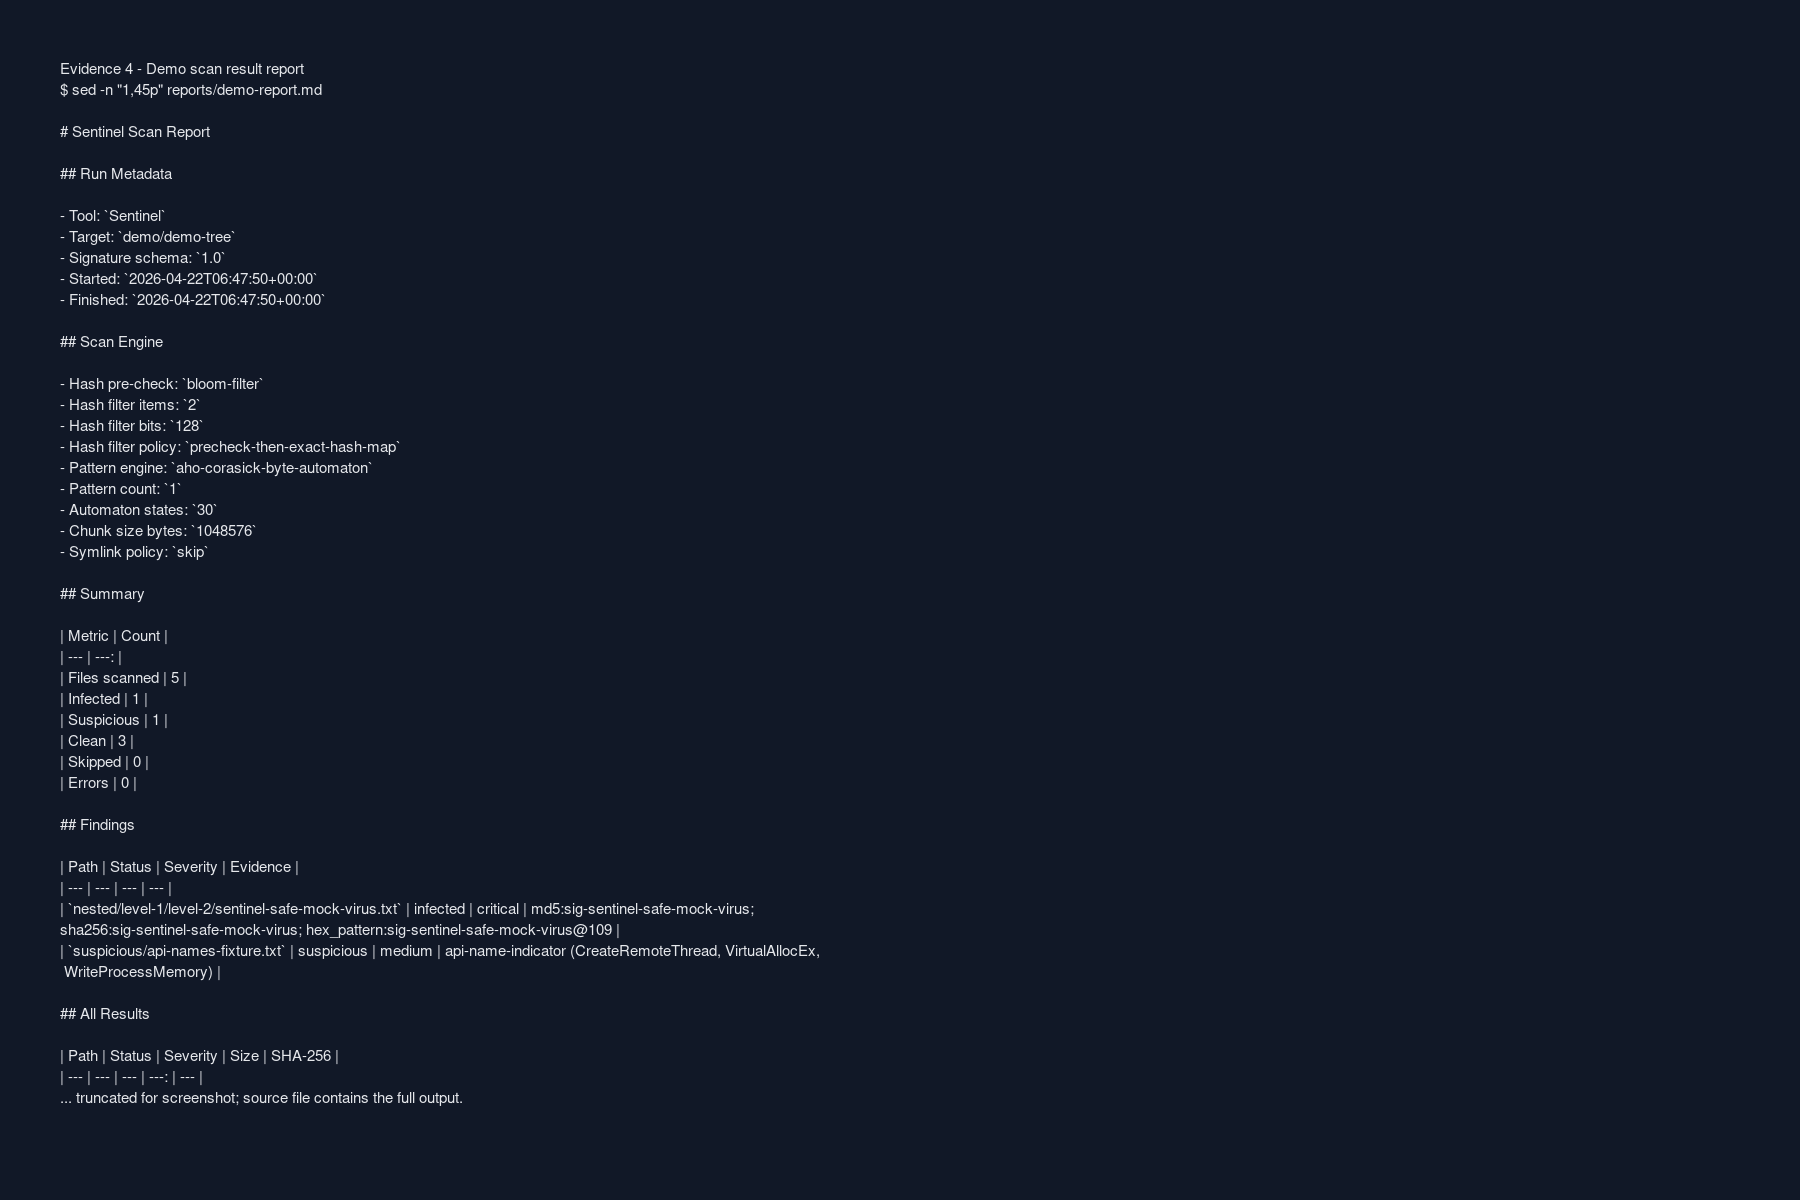
\includegraphics[width=\linewidth]{demo-report.png}
\caption{Demo report evidence showing the scan metadata, summary, and finding rows.}
\end{figure}
\clearpage

\begin{figure}[H]
\centering
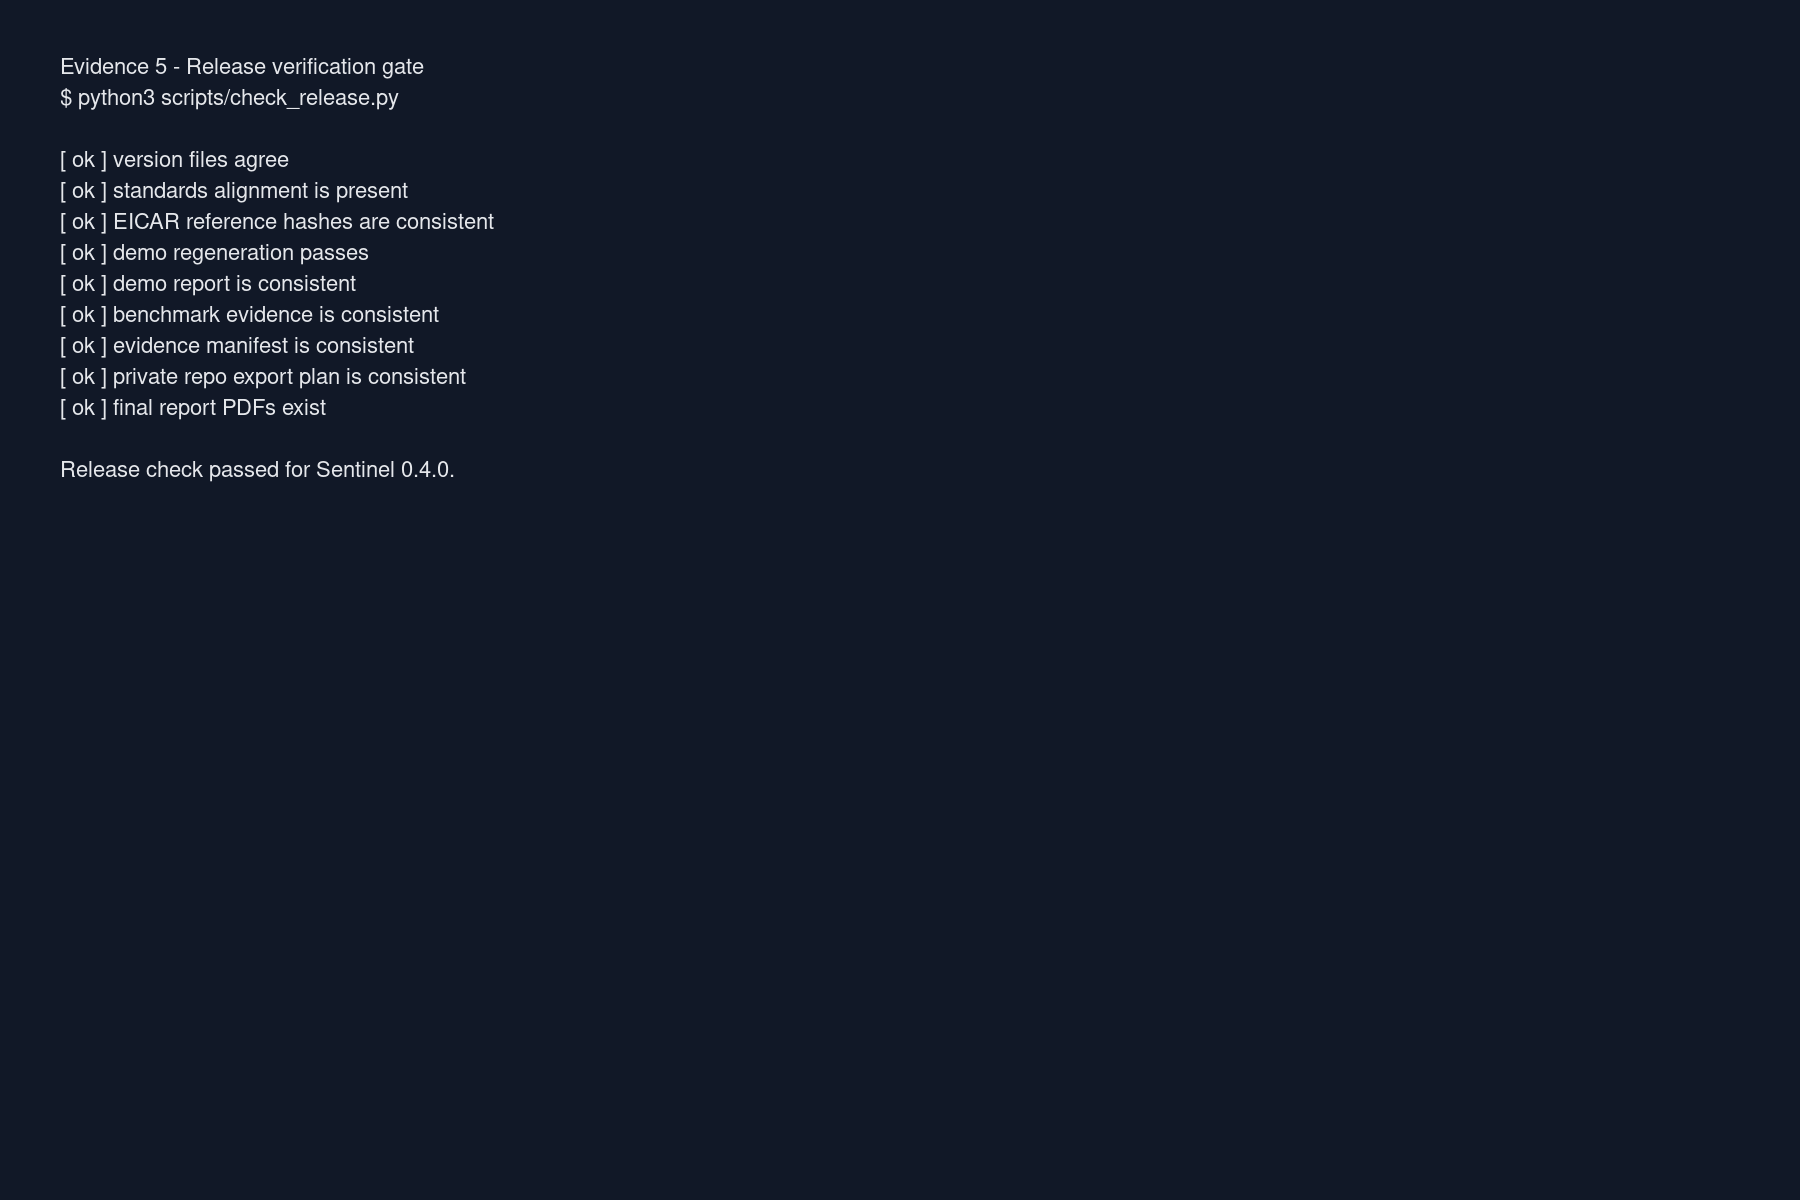
\includegraphics[width=\linewidth]{release-gate.png}
\caption{Release gate evidence showing the local release-readiness check passing.}
\end{figure}
\clearpage

\begin{figure}[H]
\centering
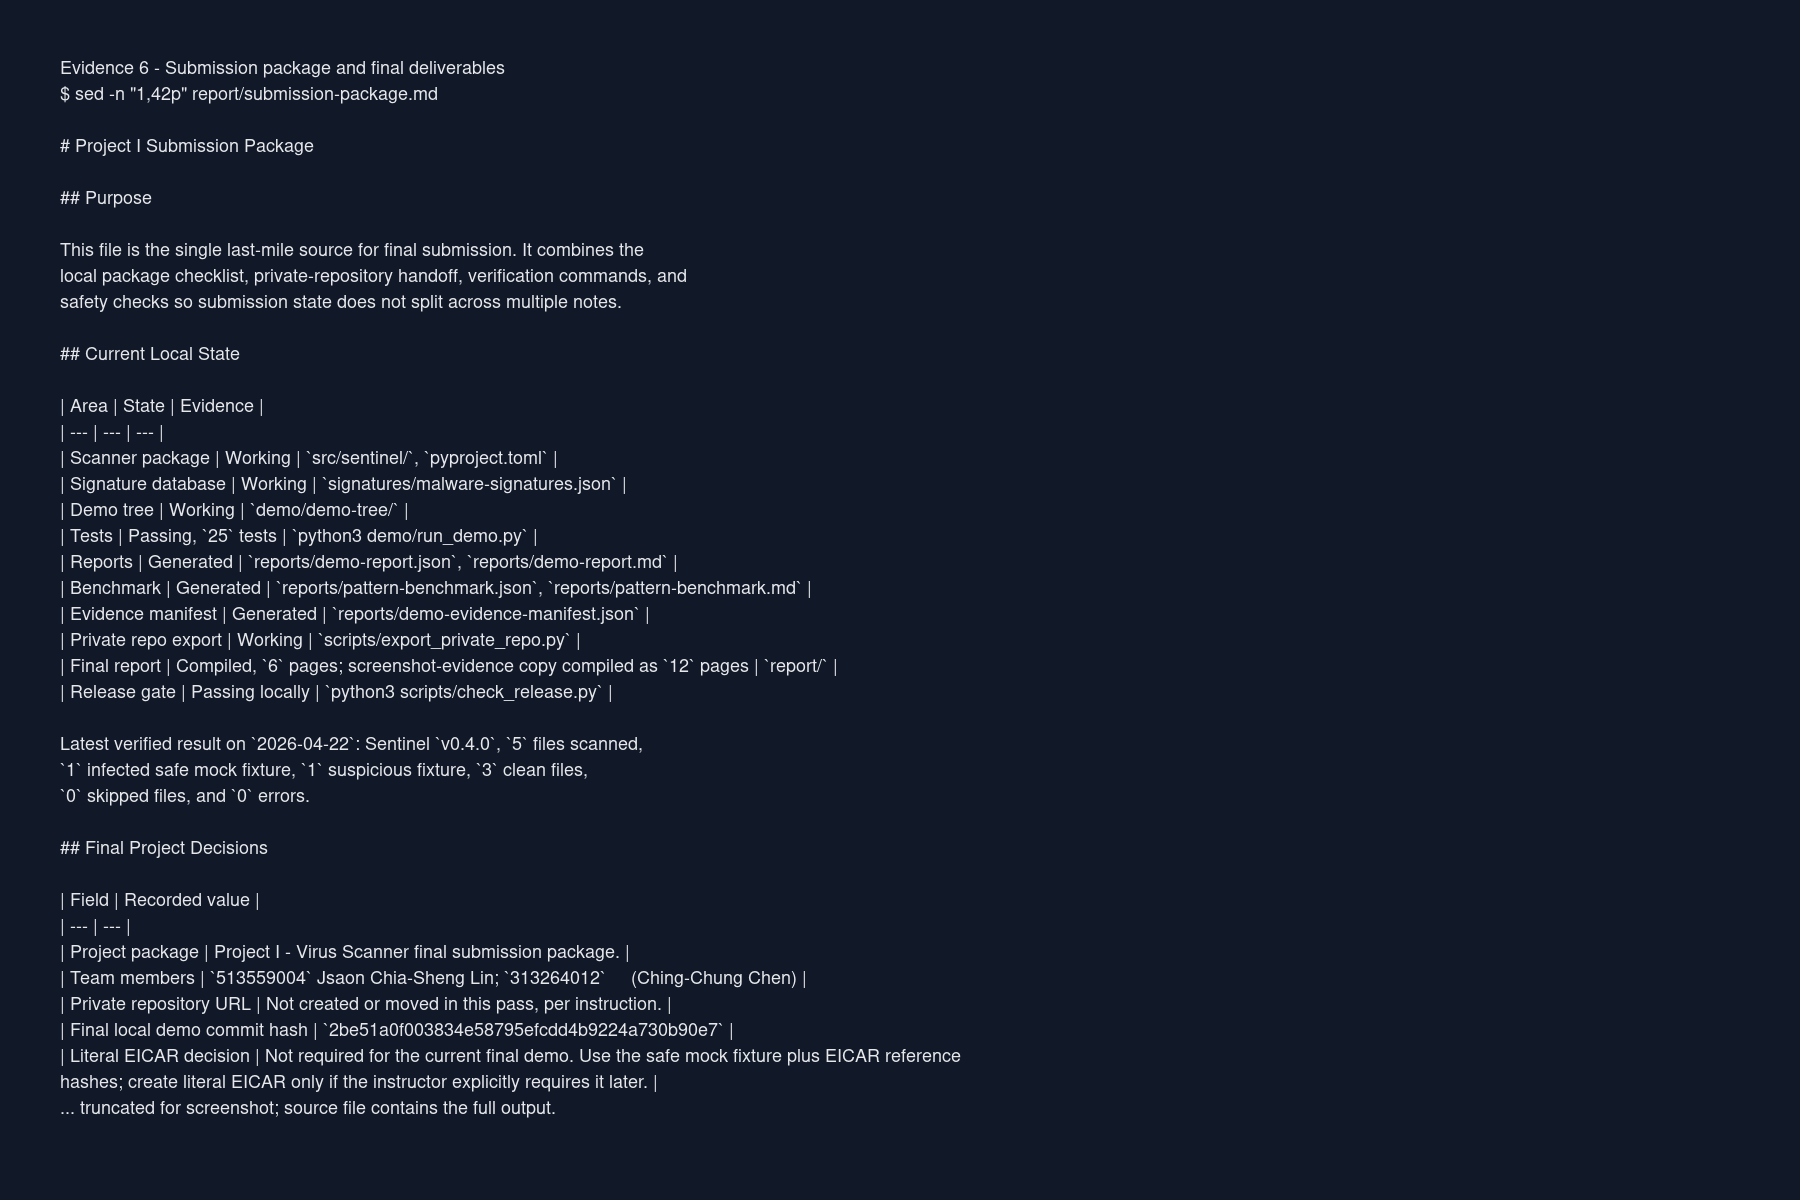
\includegraphics[width=\linewidth]{submission-package.png}
\caption{Submission package evidence showing the final deliverable checklist and recorded team fields.}
\end{figure}
\clearpage

\section{Reproduction Commands}

The main reproducibility path is:

\begin{lstlisting}[style=sentinel]
python3 demo/run_demo.py
\end{lstlisting}

This command runs the tests, validates both signature files, regenerates JSON and
Markdown scan reports, regenerates the synthetic benchmark, and regenerates the
evidence manifest. The final consistency check is:

\begin{lstlisting}[style=sentinel]
python3 scripts/check_release.py
\end{lstlisting}

Before moving the package into the required private repository, the curated
handoff folder can be generated with:

\begin{lstlisting}[style=sentinel]
python3 scripts/export_private_repo.py --clean
\end{lstlisting}

The project includes \texttt{pyproject.toml}, so it can also be installed in
editable mode with \texttt{python3 -m pip install -e .}. After installation, the
\texttt{sentinel} console command is available for the same scan, validation,
summary, and evidence-manifest workflows.

\section{Limitations And Ethics}

Sentinel is not production antivirus software. It detects only signatures and
simple heuristic indicators included in the configured database and rules. It
does not execute files, detonate samples, collect telemetry, or process live
malware. The current mock-virus fixture demonstrates scanner mechanics rather
than real-world malware coverage. The repository does not store the literal
EICAR test file; it stores only reference hashes and in-memory tests. The
benchmark is safe synthetic evidence for algorithm explanation, not a production
antivirus performance claim.

\end{document}
